%\setcounter{partie}{0} % Pour s'assurer que le compteur de \partie est à zéro dans les corrigés
% \phantom{rrr}
La figure 2 est le début d'un agrandissement de la figure 1.

Compléter la figure.

\medskip
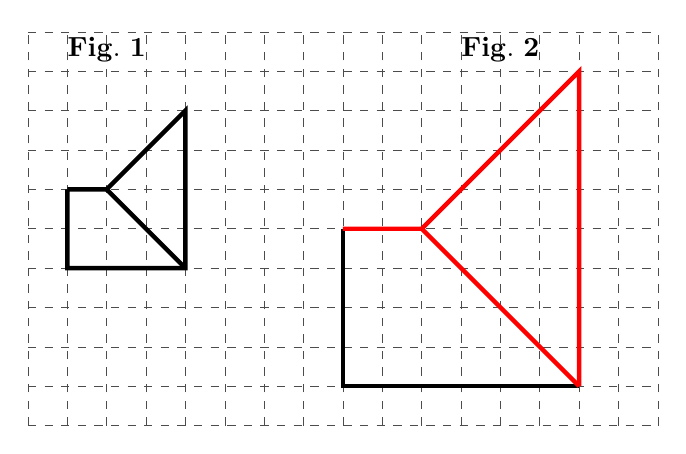
\begin{tikzpicture}[scale = 0.5]
        \draw[help lines, color=black!70, dashed] (0,0) grid (16,10);
        % Fig1
        \coordinate (A) at (1,6);
        \coordinate (B) at (2,6);
        \coordinate (C) at (4,8);
        \coordinate (E) at (4,4);
        \coordinate (F) at (1,4);
        \draw[ultra thick] (A)--(B)--(C)--(E)--(F)--(A);
        \draw[ultra thick] (B)--(E);
        \coordinate[label=above:$\mathbf{Fig.~1}$] (F1) at (2,9);
        \tkzLabelPoints[above](A,B,C);
        \tkzLabelPoints[below](E,F);
        % Fig2
        \coordinate (A') at (8,5);
        \coordinate (B') at (10,5);
        \coordinate (C') at (14,9);
        \coordinate (E') at (14,1);
        \coordinate (F') at (8,1);
        \draw[ultra thick] (E')--(F')--(A');
        \draw[ultra thick,color=red] (A')--(B')--(C')--(E');
        \draw[ultra thick,color=red] (B')--(E');
        \coordinate[label=above:$\mathbf{Fig.~2}$] (F2) at (12,9);
        \tkzLabelPoints[above](A');
        \tkzLabelPoints[below](E',F');
        \tkzLabelPoints[above,color=red](B',C');
\end{tikzpicture}

